% Chapter 1

\chapter{Introducción general} % Main chapter title

\label{Chapter1} % For referencing the chapter elsewhere, use \ref{Chapter1} 
\label{IntroGeneral}

En este capítulo se exponen los aspectos fundamentales del trabajo, con el propósito de familiarizar al lector con las estrategias de desarrollo que se detallan en los capítulos subsiguientes.

%----------------------------------------------------------------------------------------

% Define some commands to keep the formatting separated from the content 
\newcommand{\keyword}[1]{\textbf{#1}}
\newcommand{\tabhead}[1]{\textbf{#1}}
\newcommand{\code}[1]{\texttt{#1}}
\newcommand{\file}[1]{\texttt{\bfseries#1}}
\newcommand{\option}[1]{\texttt{\itshape#1}}
\newcommand{\grados}{$^{\circ}$}

%----------------------------------------------------------------------------------------

%\section{Introducción}

%----------------------------------------------------------------------------------------

\section{Descripción del proyecto}
\label{sec:desc_general}

A continuación, se presenta una descripción del contexto, problema y propuesta de solución que guiaron el presente trabajo.

\subsection{Contexto y problema}

Una cadena de supermercados en Colombia tiene importantes retos logísticos a la hora de abastecer las tiendas distribuidas en todas las ciudades. La empresa implementa centros de abastecimiento que cubren distintas ciudades en determinados rangos de acción. Uno de los retos más relevantes a los que se enfrenta, es la distribución de alimentos en cadena de frío. Dicha tarea, se lleva a cabo a través de cavas móviles que tienen la capacidad de conservar la temperatura interna y refrigerar su interior. Estas cavas representan un activo costoso y son totalmente reutilizables. En la figura \ref{fig:cava}, se puede apreciar un ejemplo de cava móvil para transporte de alimentos. 

\vspace{1cm}

\begin{figure}[htbp]
	\centering
	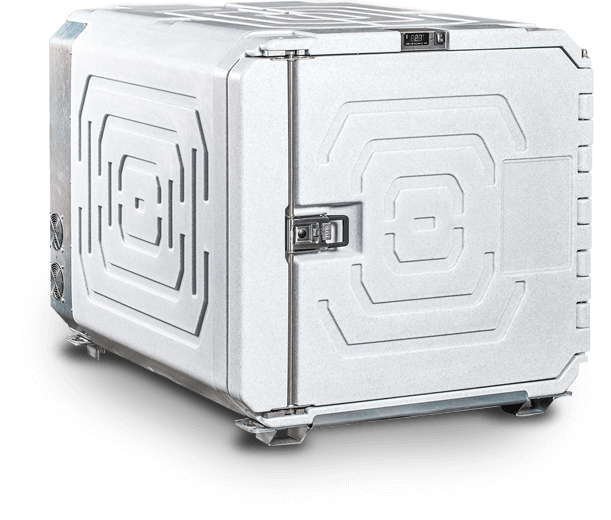
\includegraphics[width=.5\textwidth]{./Figures/cava.png}
	\caption{Ejemplo de una cava móvil\protect\footnotemark.}
	\label{fig:cava}
\end{figure}
\footnotetext{\url{https://www.coldtainer.es}}

El centro de despacho enfrenta problemas logísticos cuando se queda sin cavas disponibles para la distribución. En esta situación, es necesario realizar un esfuerzo adicional para ubicar y recuperar las cavas. La dificultad radica en que no es posible saber su ubicación exacta en tiempo real. Por lo tanto, se requiere solicitar a cada sucursal el reporte de cavas disponibles para su retorno al centro de distribución.

\subsection{Alternativa de solución}

Por lo anterior, se planteó como una alternativa de solución, el desarrollo de un dispositivo que permita rastrear la ubicación de cada una de las cavas. Este dispositivo permite replicarse con facilidad, es de bajo consumo de energía y tiene una precisión de diez metros en el reporte de ubicación de las cavas. 


%----------------------------------------------------------------------------------------

\section{Estado del arte}
\label{sec:estado_del_arte}

Los sistemas de navegación por satélite son actualmente las herramientas por excelencia en las aplicaciones de movilidad y transporte. El geo-posicionamiento es una utilidad necesaria en todos los tipos de transporte: navegación espacial, la aviación, la navegación marítima, los ferrocarriles y el transporte automotor por carretera \citep{GNSS-Junta-Adalucia}.

Uno de los sistemas de navegación más conocidos es el Sistema de Posicionamiento Global (GPS), desarrollado por el Departamento de Defensa de Estados Unidos. Sin embargo, a nivel mundial existen varios de estos sistemas, y al conjunto de ellos se le conoce como Sistemas de Navegación Global por Satélite (GNSS, del inglés Global Navigation Satellite Systems) \citep{GNSS-ONU}. Los GNSS están compuestos por constelaciones de satélites que orbitan la Tierra y transmiten datos sobre su ubicación espacial y temporal. Además, incluyen redes de estaciones de control terrestres y receptores que calculan las posiciones en tierra mediante la técnica de trilateración \citep{GNSS-ONU}. 

Algunos de los GNSS que existen actualmente son \citep{GNSS-Junta-Adalucia}:

\begin{itemize}
    \item El Sistema GPS (Global Position System): de EE. UU., con 30 satélites, a una altura de 20 200 km.
    \item El Sistema Glonass (Global Orbiting Navigation Satellite System): de Rusia, con 24 satélites, a una altura de 25 500 km.
    \item El Sistema Galileo (ESA): de Europa, con 30 satélites, a una altura de 23 200 km.
    \item El Sistema BeiDou (BDS): de China, con 34 satélites, a una altura entre 21 600 km. y 35 800  km.
\end{itemize}

En la literatura científica, estos sistemas son ampliamente estudiados y revisados, debido a su gran rango de aplicaciones en diferentes áreas del conocimiento (aparte de la navegación) y la técnica. Entre las más relevantes se destacan:

\begin{itemize}
    \item Ingeniería Civil y Arquitectura. Por ejemplo, para el replanteo de infraestructuras y estructuras, control del movimiento de tierras, medición de perfiles transversales, entre otras.
    \item Cartografía y Topografía, para mejorar la precisión de la cartografía y la modelización del mundo físico, desde montañas y ríos, hasta calles, edificios, cables y tuberías de los servicios públicos.
    \item Geodesia y Geofísica, para mejorar la precisión en el estudio de los fenómenos físicos que afectan la forma y dimensiones de la Tierra.
    \item Agricultura en el desarrollo de mejores técnicas para la gestión de los cultivos. 
\end{itemize}

\subsection{Antecedentes}

A continuación, se presentan algunos antecedentes en la literatura científica sobre el estudio de los sistemas GNSS. 

\textit{Di Garzia et al.} \citep{DiGrazia} evaluaron el rendimiento del chip receptor de GNSS TeseoV STA8135GA, de STMicroelectronics. Su trabajo se contextualiza en las aplicaciones automotrices de alta precisión. Determinaron la viabilidad técnica y las ventajas de que en un solo chip se pudiera incorporar la capacidad de recibir señales de tres bandas. Lo anterior, permitió agregar resiliencia y redundancia en caso de fallas completas de alguna de las bandas de frecuencia. 

\textit{Shu et al.}  \citep{Shu} evaluaron el rendimiento de un GNSS multi-constelación para averiguar el impacto en la determinación de la posición en un ambiente dinámico. Lo anterior, para saber cuánto mejora el GNSS la precisión de la posición. Con su estudio determinaron que:

\begin{itemize}
    \item En un caso estático, los sistemas GPS, GLONASS y BeiDou tienen el mismo rendimiento.
    \item En el caso dinámico, los sistemas GPS y GLONASS tienen rendimientos muy similares, donde el de GPS es superior. 
    \item Cuando se combinan GPS, BeiDou, GLONASS y Galileo, la respuesta es significativamente mejor en comparación con el empleo de un único sistema de posicionamiento. 
\end{itemize}

Por su parte, \textit{Villien y Denis} \citep{Villien} emplean una combinación de tres estrategias para mejorar la calidad de la recepción GNSS:

\begin{enumerate}
    \item Utilizan un receptor GNSS de múltiples constelaciones y para ampliar el rango de transmisores satelitales de los que obtener información de posicionamiento. 
    \item Utilizan una antena de banda ultra ancha (UWB, del inglés ultra-wideband) para optimizar en una única antena la capacidad de recibir señales GNSS con un ancho de banda amplio.
    \item Emplean una unidad de medida inercial junto con un filtro Kalman. Esta configuración permite rastrear de forma completa el objeto observado y reducir la carga computacional del sistema.
\end{enumerate}

El trabajo de \textit{Villien y Denis} logra un posicionamiento con una precisión de alcance entre 3 cm y 11 cm en entornos controlados. Además, se evidencia una precisión horizontal en las mediciones GNSS superior a 40 cm durante una prueba de campo, incluso en condiciones degradadas de recepción de la señal GNSS. Este trabajo es especialmente relevante en aplicaciones de geo-posicionamiento en espacios cerrados o túneles, donde un único sistema GNSS resulta insuficiente. 




%----------------------------------------------------------------------------------------

\section{Objetivos y alcance}
\label{sec:objetivos}

\subsection{Objetivo general} 

Desarrollar un prototipo de dispositivo de geolocalización basado en tecnología GNSS, que permita reportar y hacer seguimiento en tiempo real de la posición geográfica de una cava móvil de transporte de alimentos con una precisión mínima de diez metros.


\subsection{Objetivos específicos} 

\begin{enumerate}
    \item Diseñar la arquitectura de hardware y firmware, del dispositivo de geolocalización con tecnología GNSS. 
    \item Implementar el hardware y el firmware del dispositivo de geolocalización.
    \item Implementar un servicio online basado en la API de Google, para el seguimiento de la posición geográfica.
    \item Realizar pruebas de consumo energético, precisión y funcionalidad del prototipo.
\end{enumerate}


\subsection{Alcance} 

Este trabajo abordó:
\begin{itemize}
    \item El análisis de métodos ingenieriles adecuados y tecnologías disponibles para la implementación del sistema.
    \item El diseño y prototipado del sistema y subsistemas de hardware requerido para la interconexión con los sistemas GNSS, la red celular y la conexión con redes de área local a través de Wi-Fi. 
    \item El diseño y prototipado del sistema y subsistemas de hardware requerido para la interfaz humano-máquina tales como pilotos, teclas o pantallas. 
    \item El desarrollo del firmware necesario para ejecutar las funciones de conectividad, funciones lógicas y reporte de estados.
    \item Configuración de la API web necesaria para realizar pruebas de seguimiento en tiempo real del dispositivo. 
    \item Pruebas de consumo de energía. 
    \item Optimización del consumo de energía a través de firmware.
\end{itemize}

Este trabajo no incluyó:

\begin{itemize}
    \item El desarrollo de una interfaz web a medida.
    \item El diseño del aspecto físico del dispositivo. 
\end{itemize}



%----------------------------------------------------------------------------------------